\chapter{Background}
\label{chap:bg}
In this chapter, we first introduce the generative probability topic.
They are the basic of our framework.

\section{Transformer}
The Transformer is essentially an Encoder-Decoder structure, traditional CNN and RNN [17] are discarded in Transformer, and the entire network structure is entirely composed of an Attention mechanism. The total computational complexity of each layer is much lower than that of RNN and CNN(see Tab. 3.1). For the path length between remote dependencies in the network. CNN needs to increase the number of convolutional layers to expand the field of view, RNN needs to be calculated one by one from 1 to n, and self-attention only needs one step of matrix calculation. Therefore, it can also be seen that self-attention can solve the long-term dependency problem better than RNN. Of course, if the amount of calculation is too large, for example, the sequence length n¿sequence dimension d, the window can also be used to limit the number of self-attention calculations.
A trainable neural network based on Transformer can be built by stacking Transformer. Trans- former uses the Attention mechanism to reduce the distance between any two positions in the sequence to a constant; secondly, it is not a sequential structure similar to RNN, so it has better parallelism and conforms to the existing GPU framework. The structure of the Transformer is shown below as Fig.~\ref{fig:transformer}.

\begin{table}[]
	\begin{tabular}{llll}
		\hline
		Layer Type                  & Complexity per Layer & Sequential Operations & Maximum Path Length \\ \hline
		Self-Attention              & O(n2 · d)            & O(1)                  & O(1)                \\
		Recurrent                   & O(n2 · d)            & O(n)                  & O(n)                \\
		Convolutional               & $O(k\cdot n\cdot d^2)$       & $O(1) $              & $O(log_k(n)$)         \\
		Self-Attention (restricted) & O(r · n · d)         & O(1)                  & O(n/r)              \\ \hline
	\end{tabular}
\label{tab:}
\end{table}

\begin{table}[!htbp]
		\begin{center}
			\renewcommand\arraystretch{1.5}
			\setlength{\tabcolsep}{7pt}
			\begin{tabular}{l | c c c c | c c c c | c c c c | c c c c}
				\toprule[1pt] 
				\multirow{2}{*}{State}		&\multicolumn{4}{c|}{MCTM}	&\multicolumn{4}{c|}{LDA}	&\multicolumn{4}{c|}{HMM}		&\multicolumn{4}{c}{Ours}\\
				\cmidrule{2-5}		\cmidrule{6-9}		\cmidrule{10-13}	\cmidrule{14-17}
				&L	&R	&V	&VT	&L	&R	&V	&VT	&L	&R	&V	&VT	&L	&R	&V	&VT\\
				\midrule[1pt]
				Left	&\textbf{.99}	&.00	&.00	&.01	&\textbf{.49}	&.44	&.00	&.06	&\textbf{.98}	&.00	&.01	&.01	
				
				&\textbf{1.0}	&.00	&.00	&.00\\
				
				Right	&.00	&\textbf{.94}	&.01	&.05	&.00	&\textbf{1.0}	&.00	&.00	&.00	&\textbf{.92}	&.08	&.00	
				
				&.00	&\textbf{.99}	&.00	&.01\\
				
				Vertical	&.00	&.00	&\textbf{.77}	&.22	&.01	&.17	&\textbf{.82}	&.00	&.02	&.01	&\textbf{.69}	&.28	
				
				&.00	&.00	&\textbf{1.0}	&.00\\
				
				Vertical-Turn	&.31	&.05	&.20	&\textbf{.43}	&.01	&.21	&.30	&\textbf{.46}	&.49	&.04	&.32	&\textbf{.15}	
				
				&.05	&.00	&.00	&\textbf{.95}\\
				\cmidrule{1-17}	
				Average Accuracy		&\textbf{.78}	&	&	&	&\textbf{.69}	&	&	&	&\textbf{.69}	&	&	&	
				
				&\textbf{.99}	&	&	&\\	%[5ex]
				
				\bottomrule[1pt] 
				
			\end{tabular}
		\end{center}
		\caption[Comparison of Classification results between our methods and others popular methods for QMUL Juction Dataset]
		{Comparison of Classification results between our methods and others popular methods for QMUL Juction Dataset: The results of MCTM, LDA and HMM are cited from ~\cite{hospedales2012video}}
		\label{tab:qmul_compare} 
\end{table}

\begin{figure}[!htbp]
	\centering
	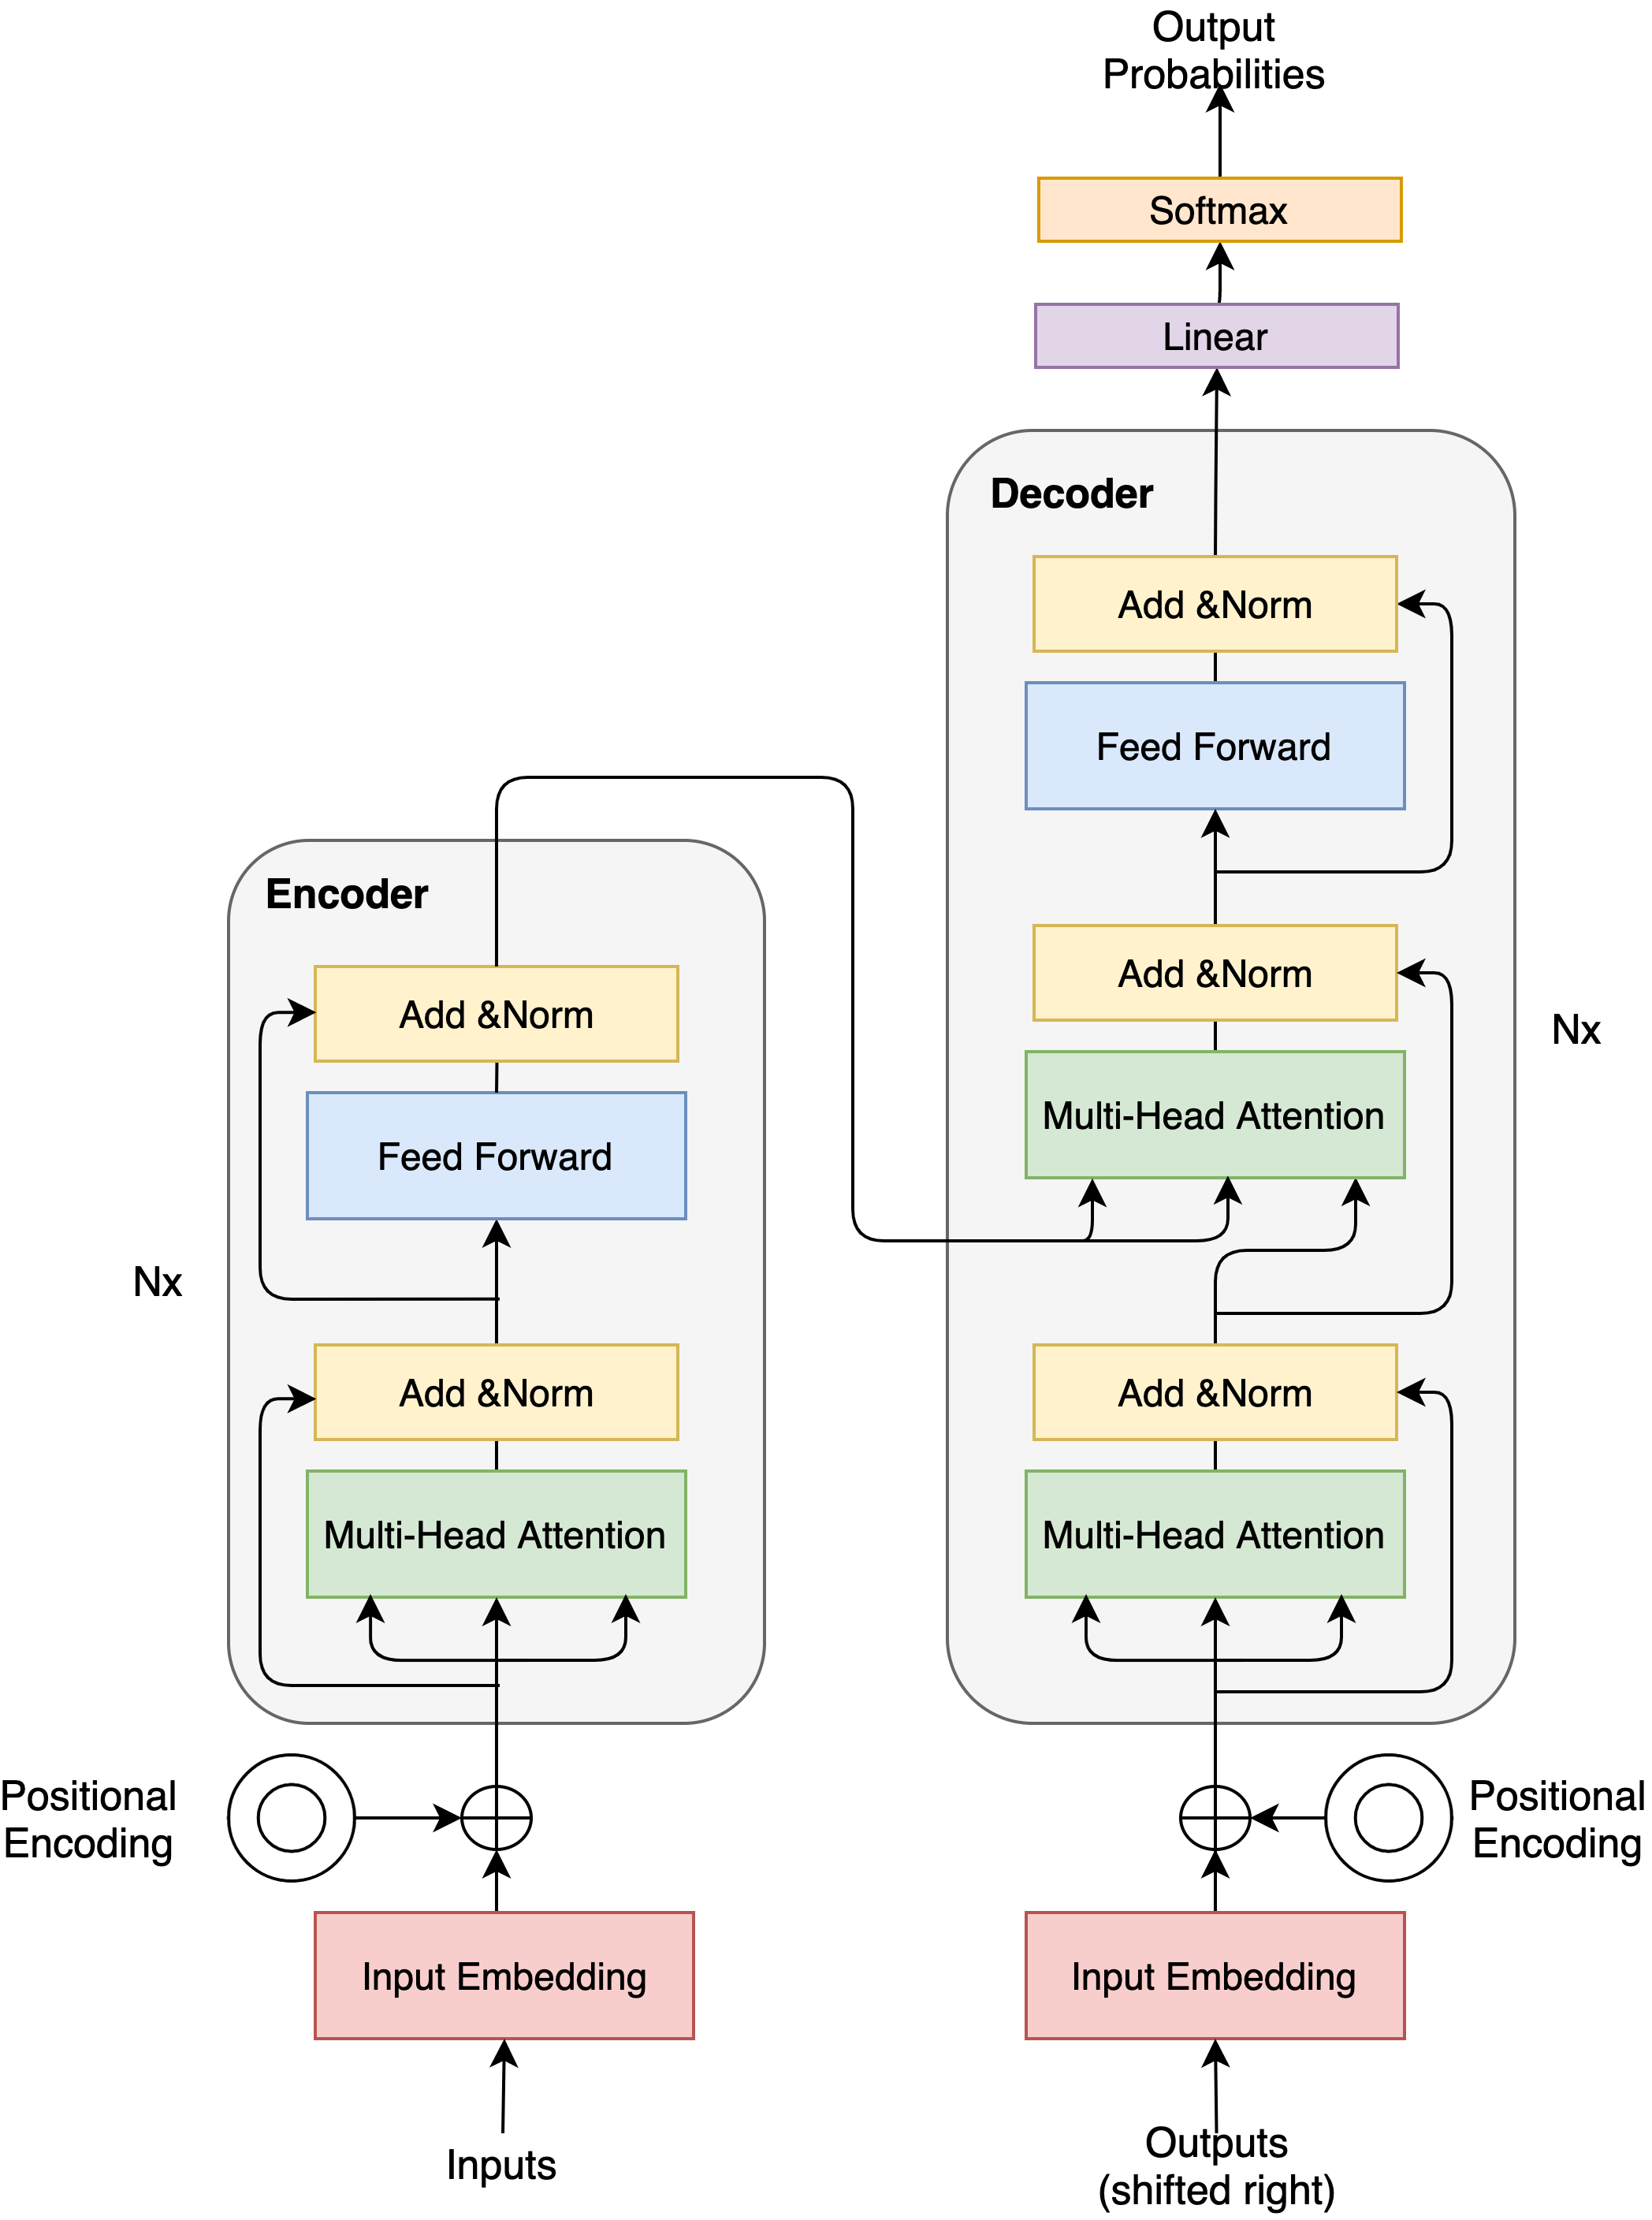
\includegraphics[width = 0.5 \textwidth]{figures/transformer.png}
	\caption[The Transformer - model architecture]
	{ The Transformer - model architecture.~\cite{vaswani2017attention}.}
	\label{fig:transformer}
\end{figure}

\subsection{Self-Attention}
Self-attention, sometimes called intra-attention is an attention mechanism relating different positions of a single sequence in order to compute a representation of the sequence. Self-attention has been used successfully in a variety of tasks including reading comprehension, abstractive summarization, textual entailment and learning task-independent sentence representations [4, 22, 23, 19].
\begin{equation}
	Attention(Q,K,V)=softmax(\frac{QK^T}{\sqrt{d_K}})V
	\label{equ:self_attention}
\end{equation}

\subsection{Multihead Attention}
\subsection{Positional Encoding}

\begin{equation*}
	\begin{aligned}
	PE_{(pos,2i)} = sin(pos/10000^{2i/d_{model}}),\\
	PE_{(pos,2i+1)} = cos(pos/10000^{2i/d_{model}})
	\end{aligned}
\end{equation*}


\section{Artificial Neural Network}
\subsection{Activation Function}
\subsection{Fully Connection Layer}
\subsection{Convolutional Layer}

\section{Ranking Loss}
